%%%%%%%%%%%%%%%%%%%%%%%%%%%%
% Prototype Implementation %
%%%%%%%%%%%%%%%%%%%%%%%%%%%%

\chapter{Prototyp-Implementierung}
\label{chapter:prototype}

\begin{figure}[hbt]
    \centering
    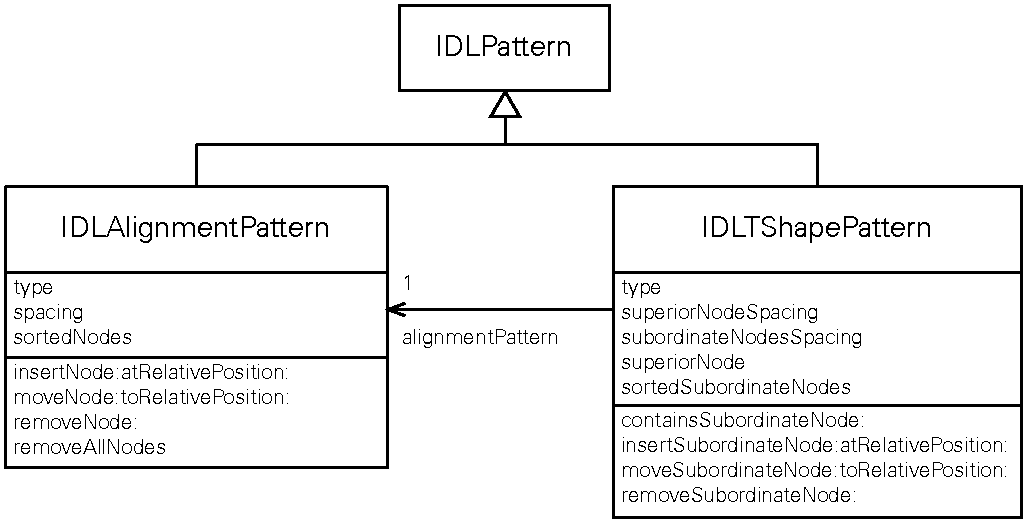
\includegraphics[width=\textwidth]{resources/layout-patterns-implementation}
    \caption{}
    \label{fig:layout-patterns-implementation}
\end{figure}

% Anforderungen an den Prototypen?

% Das Layout-Framework von Sonja Maier konnte nicht als Grundlage verwendet werden, da nicht veröffentlicht

% kurze Beschreibung des Prototypen
% unterstützte Operationen

% Präfix "IDL" erklären

% Animation der Layout-Übergängen
% - implizite Core Animation Animation
% - Überführen von mehreren Animationen mit POP

% IDLLayoutEngine besitzt intern Referenzen auf den Inhalt des Diagramms und muss daher mit dem Diagramm synchronisiert werden (manuell) mit s.g. Layout-Events
% Layout-Events auflisten und mit Bildern erklären

% Löschen eines (oder mehreren Elementen) im Prototypen nicht unterstützt, nur hinzufügen und "rausfahren"

% aus zeitlichen Gründen wurde die Semantik nicht tiefgründig ausgearbeitet und wurde der weiteren Forschung überlassen
% IDLEdge -> gerichtete Kanten mit max. einem Elternknoten (z.B. Vererbung in Klassendiagrammen) -> Diagramm ist also azyklisch

% Liste der unterstützten ästhetischen Kriterien

% Beschreibung der App, Komponenten, genutzte API's, unterstützte Layout-Methoden, Koordinaten (Umrechnung), Drag and Drop

% - IDLPattern, IDLAlignmentPattern, IDLTShapePattern -> Klassendiagramm
% Wiederverwendung, Komposition in IDLTShapePattern

% IDLLayoutEngine & Subclasses (bzw. unterstützte Layout-Engines)

% Koordinaten-Konversion mit Bild (NSView vs. IDLLayoutEngine)
% zentrierte Koordinaten -> Förderung der Umsetzung des impliziten Patterns zur Zentrierung
% Vergrößerung des Fensters -> Zentrierung des Inhalts

% wie werden die impliziten Patterns im Prototypen implementiert

% Berechnung der Start- und Endpunkte der Kanten anhand von Eigenschaften der Knoten (siehe OmniGraffle)

% Demo-Videos auf der DVD

% Vernachlässigungen
% ==================
% - kein Metamodell
% - keine Unterscheidung der abstrakten und konkreten Syntax
% - siehe Blatt "Patterns in UML Klassendiagrammen"

% Schwachstellen
% ==============
% manchmal Probleme mit Animation bei D&D
% Pattern-Abhängigkeiten müssen manuell verwaltet werden
% IDLPatternsSolver mit einem Constraint Solver

% Entwicklungspotential
% =====================
% Implementierung der Auswahl von Elementen
% Unterstützung von weiteren Operationen
% Anpassung für Klassendiagramme
